\section{Visualization}

\begin{frame}{Basic Pipeline}
    \makebox[\textwidth][c]{
    \begin{tikzpicture}[
    scale=0.9, every node/.style={scale=0.9},
fixedrect/.style={rectangle,draw,minimum height=4em,anchor=west,text width=2cm,align=center},
]
        \node[label=west:{GPU},align=right](gpu) at (0,0){};
        \node[label=west:{CPU 0},align=right](c0) at (0,-1.75){};
        \node[label=west:{CPU 1},align=right](c1) at ($(c0.west) - (0,4em)$){};

        \node[fixedrect, text width=6cm](gpu_sim) at (gpu){Simulation};%\\[CUDA]};
        \node[fixedrect, text width=3cm](gpu_viz) at (gpu_sim.east){Visualization};%\\[Vulkan]};

        \node[fixedrect, text width=6cm](c0_sim) at (c0){Manage Sim Kernels};%\\[Vulkan]};
        \node[fixedrect, text width=2cm](c1_record) at (3,0 |- c1){Record Visualization};%\\[Vulkan]};

        \draw[-latex] (c1_record.east) -| (gpu_viz.south);
        % \draw[-latex] (c1_record.east) -- (gpu_viz.south);
        % \draw[-latex] (c1_record.east) -| (gpu_viz.south);
        % \draw[-latex] (c1_record.east) -| (gpu_viz.south);
    \end{tikzpicture}
    }

    % \vfill\null
    
    \begin{wideitemize}
        \item CPU 0 manages the Simulation CUDA kernels.
        \item CPU 1 records GPU commands into Vulkan Command Buffers\todocite{}.
        \item These actions are executed once the Simulation is finished.
        \item Aim for 100\% GPU utilization.
    \end{wideitemize}
\end{frame}

\subsection{Research}
\begin{frame}{Visualization Research}
    \begin{wideitemize}
        \item No recent academic innovation $\implies$ look to industry.\todomark{Expand on this w/ evidence}
        \item How do industrial programs visualize fluid sims?
        \item Picked Autodesk CFD as reference.
        \item 3D techniques can be translated to 2D.
    \end{wideitemize}
\end{frame}

\newcommand{\vizresearch}[3]{
\begin{frame}{Visualization Research}
    \framesubtitle{What can Autodesk CFD do?}
    \begin{columns}[t,onlytextwidth]
        \begin{column}{0.5\textwidth}
            {\Large #1}
            \vspace{2em}
            #2
        \end{column}
        \begin{column}{0.5\textwidth}
            #3
            \todomark{Images}
            % \input{Images!!}
        \end{column}
    \end{columns}
\end{frame}
}

\vizresearch{Result Planes - Scalar}{
    \todocite{http://help.autodesk.com/view/SCDSE/2019/ENU/?guid=GUID-AA40D02F-8CBC-4F78-A3C8-CEF30E05522B}
    \begin{wideitemize}
        \item Place a plane in 3D space
        \item Select a scalar quantity (pressure, temperature etc.)
        \item The cross-section of the model shows the selected quantity, with a color scale \todomark{matplotlib jet colormap}
    \end{wideitemize}
}{
% \input{Images!!}
}

\vizresearch{Result Planes - Vector}{
    \todocite{http://help.autodesk.com/view/SCDSE/2019/ENU/?guid=GUID-AA40D02F-8CBC-4F78-A3C8-CEF30E05522B}
    \begin{wideitemize}
        \item Place a plane in 3D space
        \item Select a \emph{vector} quantity (velocity etc.)
        \item The cross-section of the model shows a vector field of the selected velocity.
    \end{wideitemize}
}{
% \input{Images!!}
}

\vizresearch{Isosurfaces}{
\todocite{http://help.autodesk.com/view/SCDSE/2019/ENU/?guid=GUID-9D0D1D9C-C087-42A5-87F6-24F6A8530244}
    \begin{wideitemize}
        \item Select a scalar quantity $X$.
        \item Select a value $X = x$.
        \item This surface is displayed with a color based on another quantity $Y$.
        \item A vector quantity can also be added to the surface.
    \end{wideitemize}
}{
% \input{Images!!}
}

\vizresearch{Isovolumes}{
\todocite{http://help.autodesk.com/view/SCDSE/2019/ENU/?guid=GUID-9D0D1D9C-C087-42A5-87F6-24F6A8530244}
    \begin{wideitemize}
        \item Select a scalar quantity $X$.
        \item Select a \emph{range} $x_{min} \leq X \leq x_{max}$.
        \item This \emph{volume} is displayed with a color based on another quantity $Y$.
        \item A vector quantity can also be added to the \emph{volume}.
    \end{wideitemize}
}{
% \input{Images!!}
}

\vizresearch{Particles}{
\todocite{http://help.autodesk.com/view/SCDSE/2019/ENU/?guid=GUID-9EBC3C73-AB3B-4341-BBDF-58601024BD7C}
    \begin{wideitemize}
        \item Place particle spawn points (`seeds').
        \item Select a scalar quantity to display, or a solid color.
        \item Points along the particle paths show the specified quantity.
        \item Can choose many kinds of path:
        \begin{itemize}
            \item Cylinders
            \item Ribbons
            \item Comets
            \item etc.
        \end{itemize}
    \end{wideitemize}
}{
% \input{Images!!}
}

\begin{frame}{Our Selection}
    % \mytwocolumn{0.5}{
        Separate the visualization into layers:
        \vspace{1em}

        \begin{wideitemize}
            \item Background
            \item Scalar Quantity
            \begin{itemize}
                \item Display a quantity $X$ using a colormap when $x_{min} \leq X \leq x_{max}$
                \item Allow the user to select a range, or calculate a range containing all values
                \item Equivalent to Results Plane (Scalar) + Isovolume
            \end{itemize}
            \item Vector Quantity 
            \begin{itemize}
                \item Display a vector field of $X$ when $x_{min} \leq X \leq x_{max}$
                \item Allow the user to select a range, or calculate a range containing all values
                \item Equivalent to Results Plane (Vector) + Isovolume
            \end{itemize}
            \item Particles
                \begin{itemize}
                    \item Editable `seeds'
                    \item Planned for particle trace options, didn't have time.
                \end{itemize}
        \end{wideitemize}
    % }{
    % daui
    % }
\end{frame}

\usetikzlibrary{shapes}
\newcommand{\tikzstaggeredgrid}[1]{
    \draw[#1] (0, 1) -- (6, 1);
    \draw[#1] (0, 3) -- (6, 3);
    
    \draw[#1] (1,4) -- (1,0);
    \draw[#1] (3,4) -- (3,0);
    \draw[#1] (5,4) -- (5,0);
    
    % \node at (0, 0.5) {j-1}; 
    % \node at (0, 2) {j}; 
    % \node at (0, 3.5) {j+1};
    
    % \node at (0.5, 0) {i-1}; 
    % \node at (2, 0) {i}; 
    % \node at (4, 0) {i+1};
    % \node at (5.5, 0) {i+2};
    
    \node[label=above:{$p_{i,j}$}, draw, circle, fill, minimum size=0.12cm, inner sep=0pt] at (2, 2) {};
    \node[label=above:{$p_{i+1,j}$}, draw, circle, fill, minimum size=0.12cm, inner sep=0pt] at (4, 2) {};
    
    \node[label=below left:{$u_{i-1,j}$}, draw, diamond, fill, minimum size=0.14cm, inner sep=0pt] at (1, 2) {};
    \node[label=below left:{$u_{i,j}$}, draw, diamond, fill, minimum size=0.14cm, inner sep=0pt] at (3, 2) {};
    \node[label=below right:{$u_{i+1,j}$}, draw, diamond, fill, minimum size=0.14cm, inner sep=0pt] at (5, 2) {};
    
    \node[label=above:{$v_{i,j}$}, draw, rectangle, fill, minimum size=0.1cm, inner sep=0pt] at (2, 3) {};
    \node[label=above:{$v_{i+1,j}$}, draw, rectangle, fill, minimum size=0.1cm, inner sep=0pt] at (4, 3) {};
    \node[label=below:{$v_{i,j-1}$}, draw, rectangle, fill, minimum size=0.1cm, inner sep=0pt] at (2, 1) {};
    \node[label=below:{$v_{i+1,j-1}$}, draw, rectangle, fill, minimum size=0.1cm, inner sep=0pt] at (4, 1) {};
}
\begin{frame}{Required Simulation Data}
    % \mytwocolumn{0.5}{
        \begin{wideitemize}
            \item Simulation stores data on a staggered grid
            \item Visualization wants to get data at specific points
            \item Convert the Simulation data to a Texture, which has dedicated sampling hardware on the GPU.
        \end{wideitemize}
    % }{
        \begin{center}
            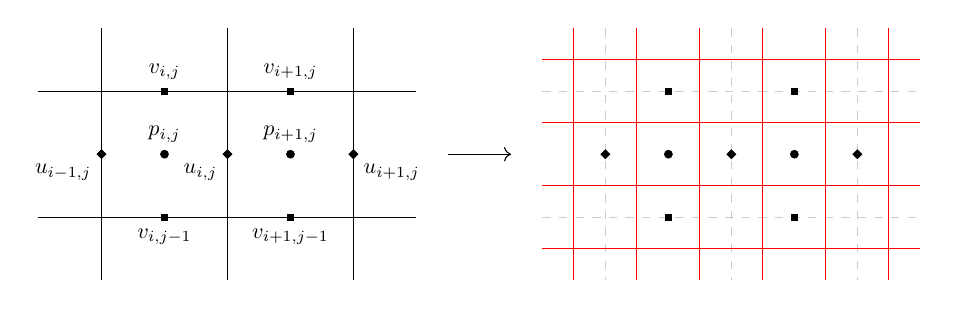
\begin{tikzpicture}[scale=0.8,every node/.style={scale=0.8},]
                \tikzstaggeredgrid{}
                
                \draw[->](6.5, 2) -- (7.5, 2);
                
                \begin{scope}[shift={(8,0)},every label/.append style={text opacity=0}]
                    \tikzstaggeredgrid{dashed,opacity=0.2}
                    
                    \draw[red] (0, 0.5) -- (6, 0.5);
                    \draw[red] (0, 1.5) -- (6, 1.5);
                    \draw[red] (0, 2.5) -- (6, 2.5);
                    \draw[red] (0, 3.5) -- (6, 3.5);

                    \draw[red] (1.5,4) -- (1.5,0);
                    \draw[red] (2.5,4) -- (2.5,0);
                    \draw[red] (3.5,4) -- (3.5,0);
                    \draw[red] (0.5,4) -- (0.5,0);
                    \draw[red] (4.5,4) -- (4.5,0);
                    \draw[red] (5.5,4) -- (5.5,0);
                \end{scope}
            \end{tikzpicture}
        \end{center}
    % }
\end{frame}

\newcommand{\vizpipeline}{
    \node[label=west:{Preprocessing},align=right](preproc) at (0,1.5){};
    \node[label=west:{Scalar Quantity},align=right](sq) at (0,0){};
    \node[label=west:{Vector Quantity},align=right](vq) at (0,-1.5){};
    \node[label=west:{Particles},align=right](p) at (0,-3){};
    
    \node[fixedrect](preproc_c1) at (preproc){Extract Data Texture};
    
    % \node[fixedrect](sq_prelim) at (0, 1){Convert arrays to image};
    \node[fixedrect](sq_c1) at (sq){Extract Quantity};
    \node[fixedrect](sq_c2) at (sq_c1.east){Find min/max\\(Optional)};
    
    \node[fixedrect](vq_c1) at (vq){Extract Quantity};
    \node[fixedrect](vq_c2) at (vq_c1.east){Find min/max\\(Optional)};
    \node[fixedrect](vq_c3) at (vq_c2.east){Create Vector Instances};
    
    \node[fixedrect](p_c1) at (p){Decide Particles to emit};
    \node[fixedrect](p_c2) at (p_c1.east){Emit new Particles};
    \node[fixedrect](p_c3) at (p_c2.east){Simulate Particles};
    
    \node[fixedrect](sq_r) at (10.5, 0){Draw\\Background w/ Quantity};
    \node[fixedrect](vq_r) at (sq_r.west |- vq){Draw\\Vector Instances};
    \node[fixedrect](p_r) at (sq_r.west |- p){Draw\\Particles};
    
    \draw [decorate,decoration={brace,raise=5pt,amplitude=7pt,mirror},yshift=-20pt](sq_c1.west |- p_r.south) -- (p_c3.east |- p_r.south) node [black,midway,anchor=north,below=15pt]{Compute};
    
    \draw [decorate,decoration={brace,raise=5pt,amplitude=7pt,mirror},yshift=-20pt](sq_r.west |- p_r.south) -- (p_r.east |- p_r.south) node [black,midway,anchor=north,below=15pt]{Graphics};
}

\begin{frame}{Visualization Pipeline}
    \makebox[\textwidth][c]{
    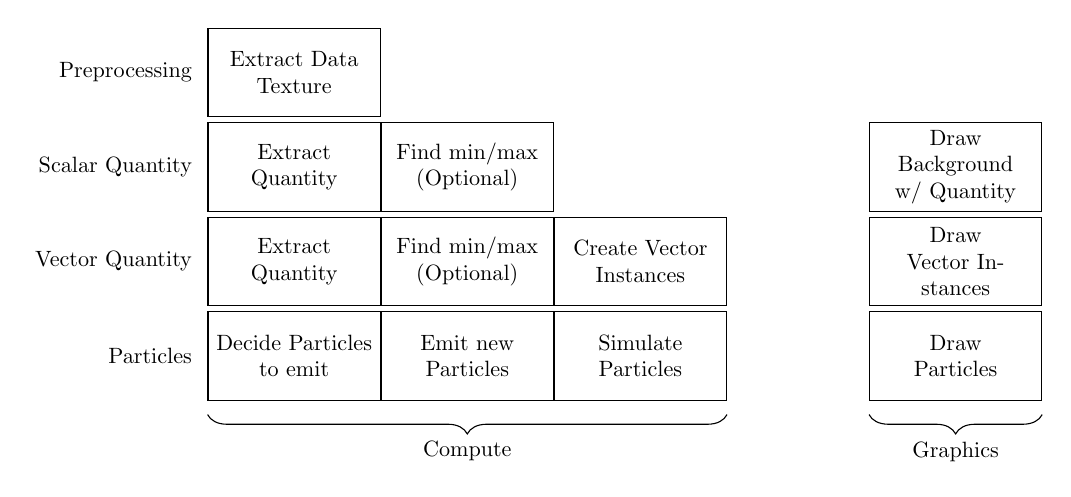
\begin{tikzpicture}[
    scale=0.8, every node/.style={scale=0.8},
fixedrect/.style={rectangle,draw,minimum height=4em,anchor=west,text width=2.5cm,align=center},
]   
        \vizpipeline{}
    \end{tikzpicture}
    }

    Each layer requires both compute work and graphics work.
\end{frame}

\begin{frame}[t]{Visualization Pipeline}
    \makebox[\textwidth][c]{
    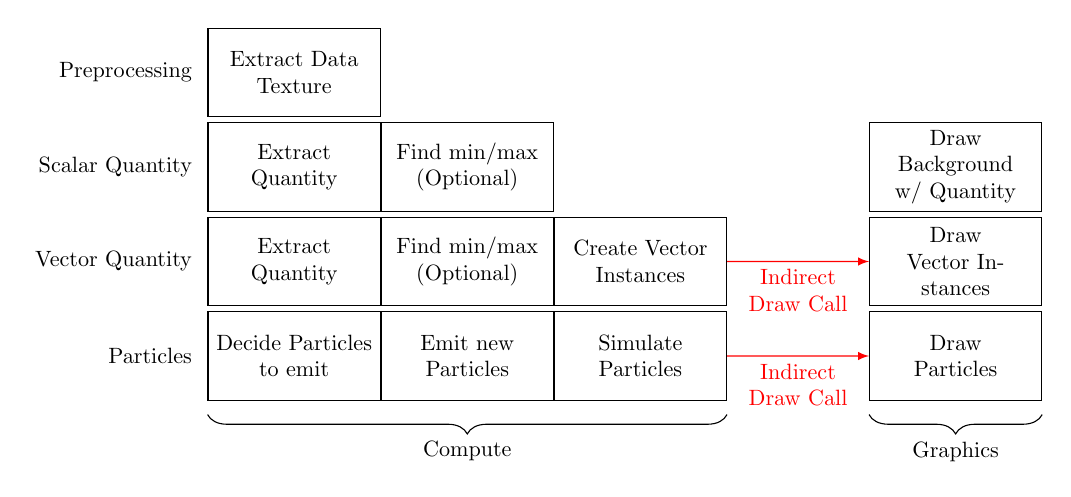
\begin{tikzpicture}[
    >=latex,
    scale=0.8, every node/.style={scale=0.8},
fixedrect/.style={rectangle,draw,minimum height=4em,anchor=west,text width=2.5cm,align=center},
]   
        \vizpipeline{}
        
        \begin{scope}[overlay]
            \draw[red,-latex] (p_c3.east) -- (p_r.west) node [red,midway,below,text width=3cm,align=center]{Indirect\\Draw Call};
            \draw[red,-latex] (vq_c3.east) -- (vq_r.west) node [red,midway,below,text width=3cm,align=center]{Indirect\\Draw Call};
        \end{scope}
    \end{tikzpicture}
    }
    \vfill\null
    
    When recording, we don't know how many particles exist.
    
    Use \textbf{Indirect Instanced Rendering} to allow the Compute phase to control how many particles are drawn.
    % The number of vectors and particles that are drawn isn't defined until the Compute is finished, so they are drawn using \textbf{Indirect Instanced Rendering}.
    
    % The Compute phase fills a buffer with data on how many things to render, and the GPU reads from this when it starts rendering.
\end{frame}

\usetikzlibrary{fadings}
\begin{frame}{GPU Pipeline}
\begin{figure}[t]
    \makebox[\textwidth][c]{
    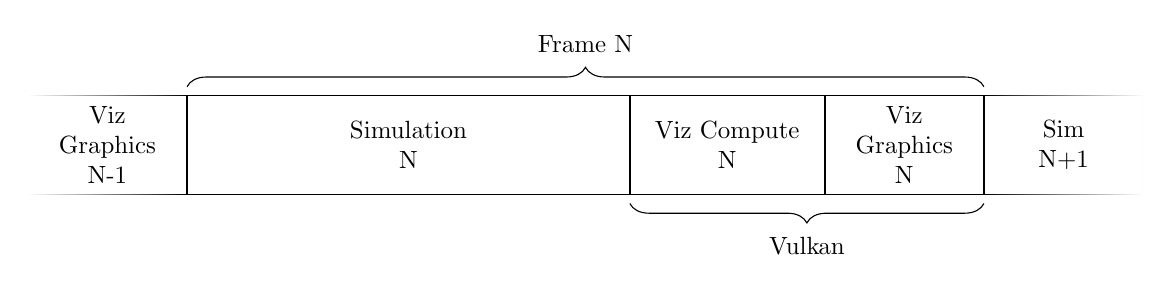
\begin{tikzpicture}[
    scale=0.9, every node/.style={scale=0.9},
fixedrect/.style={rectangle,draw,minimum height=4em,anchor=west,text width=2cm,align=center},
]
        \node[fixedrect, text width=6cm](sim) at (0,0){Simulation\\N};%\\[CUDA]};
        \node[fixedrect, text width=2.5cm](vc) at (sim.east){Viz Compute\\N};%\\[Vulkan]};
        \node[fixedrect, text width=2cm](vg) at (vc.east){Viz Graphics\\N};
        
        \node[fixedrect, text width=2cm, anchor=east,path fading = west] at (sim.west){Viz Graphics\\N-1};
        \node[fixedrect, text width=2cm, anchor=west,path fading = east] at (vg.east){Sim\\N+1};

        \draw [decorate,decoration={brace,raise=0pt,amplitude=7pt},yshift=-5pt](sim.west |- 0,1) -- (vg.east |- 0,1) node [black,midway,anchor=south,above=10pt]{Frame N};
        
        % \draw [decorate,decoration={brace,raise=0pt,amplitude=7pt,mirror},yshift=5pt](sim.west |- 0,-1) -- (sim.east |- 0,-1) node [black,midway,anchor=north,below=10pt]{CUDA};
        \draw [decorate,decoration={brace,raise=0pt,amplitude=7pt,mirror},yshift=5pt](vc.west |- 0,-1) -- (vg.east |- 0,-1) node [black,midway,anchor=north,below=10pt]{Vulkan};

    \end{tikzpicture}
    }
    \end{figure}
    
    \vfill\null
    
    \begin{wideitemize}
        \item Simulate, perform compute, then render.
        \item Wanted to overlap visualization with simulation, but my graphics card (GTX 1080) can't run multiple compute workloads at once.\footnote{RTX 3000 series are the first cards to run two compute workloads in parallel.\todocite{rtx 30 whitepaper}}
        \item Viz Graphics \emph{could} overlap with the simulation\todocite{Overlapping graphics with compute}, but this doesn't happen in practice.
    \end{wideitemize}
    
\end{frame}

\usetikzlibrary{arrows.meta}
\begin{frame}{GPU Pipeline - Synchronization I}
\begin{figure}[t]
    \makebox[\textwidth][c]{
    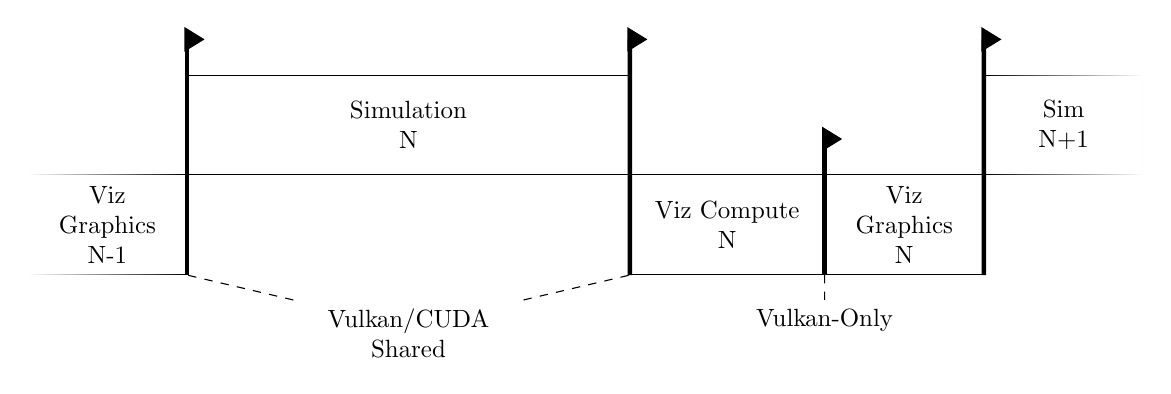
\begin{tikzpicture}[
    scale=0.9, every node/.style={scale=0.9},
fixedrect/.style={rectangle,draw,minimum height=4em,anchor=west,text width=2cm,align=center},
]
        \node[fixedrect, text width=6cm](sim) at (0,0){Simulation\\N};%\\[CUDA]};
        \node[fixedrect, text width=2.5cm](vc) at (sim.east |- 0,-4em){Viz Compute\\N};%\\[Vulkan]};
        \node[fixedrect, text width=2cm](vg) at (vc.east){Viz Graphics\\N};
        
        \node[fixedrect, text width=2cm, anchor=east,path fading = west](vg_old) at (sim.west |- vc){Viz Graphics\\N-1};
        \node[fixedrect, text width=2cm, anchor=west,path fading = east](sim_new) at (vg.east |- sim){Sim\\N+1};
        
        \draw[ultra thick,black,-Triangle] (vc.south west) -- (sim.north east) |- ++(0.25,0.5) ;
            % node[east,text width=2cm,anchor=west]{Vulkan/CUDA Shared Semaphore};
        \draw[ultra thick,black,-Triangle] (vg_old.south east) -- (sim.north west) |- ++(0.25,0.5) ;
            % node[east,text width=2cm,anchor=west]{Vulkan/CUDA Shared Semaphore};
        \draw[ultra thick,black,-Triangle] (vg.south east) -- (sim_new.north west) |- ++(0.25,0.5) ;
            % node[east]{};
            
        \draw[ultra thick,black,-Triangle] (vg.south west) -- (vg.north west) |- ++(0.25,0.5) ;
            % node[text width=2cm,anchor=north,below=5pt]{Vulkan-Only};

            
        \node[text width = 3cm,align=center,anchor=north,below=10pt](sem_label) at (sim.south |- vc.south){Vulkan/CUDA Shared};
        \draw[dashed](sem_label.north east) -- (vc.south west);
        \draw[dashed](sem_label.north west) -- (vg_old.south east);
        
        \node[text width = 3cm,align=center,anchor=north,below=10pt](vk_label) at (vg.south west){Vulkan-Only};
        \draw[dashed](vk_label.north) -- (vc.south east);

        \end{tikzpicture}
    }
    \end{figure}
    
    \vfill\null
    
    \begin{wideitemize}
        \item Synchronization between overall workloads is performed via \emph{semaphores} (GPU-GPU sync primitives)\todocite{}.
        \item Workloads wait on a semaphore until another workload signals it.
        \item More semaphores used in the program for `present' logic.
    \end{wideitemize}
    
\end{frame}

\usetikzlibrary{shapes.multipart}
\begin{frame}[t]{GPU Pipeline - Synchronization II}
\begin{figure}[t]
    \makebox[\textwidth][c]{
    \begin{tikzpicture}[
    scale=0.9, every node/.style={scale=0.9},
fixedrect/.style={rectangle,draw,minimum height=4em,anchor=west,text width=2cm,align=center},
]
        \node[fixedrect,   rectangle split,
  rectangle split parts=2,
  rectangle split horizontal,text width=6cm,
  rectangle split draw splits=false](vc1) at (0,0){Viz Compute\\N\nodepart{two}};%\\[Vulkan]};
        % \node[fixedrect, text width=4cm,path fading = east](vc2) at (vc.east){};
        \node[fixedrect,fill=white,draw=white,path fading=west,minimum width=4cm,anchor=east,minimum height=5em] at ($(vc1.east) + (0.1,0)$){};


        \end{tikzpicture}
    }
    \end{figure}
    \todomark{Rest of diagram}
    
    \vfill\null
    
    \begin{wideitemize}
        \item Simulation CUDA kernels use the same stream, so are implicitly ordered\todocite{cuda streams ordered}.
        \item Vulkan commands are not implicitly ordered\todocite{}.
        \item Use memory barriers to ensure that memory writes from one kernel are visible in the next.\footnote{This is enough to ensure they execute in order.}
    \end{wideitemize}
    
\end{frame}

% TODO - can mention VTK GPU integration here ("other projects are using GPUs!")
% Datoviz uses Vulkan

% sharing memory
% want to copy/move memory as little as possible => have vulkan read data from the CUDA buffers.
% use of allocators
% compile-time switching between using "Vulkan-capable" memory and "CUDA-capable" memory
% (vulkan-capable memory only used for data required by vulkan - fluidmask, velocity, pressure)
% (vulkan memory requirements known ahead of time, able to allocate it all at once and sub-allocate each buffer)

% Top-level - integrating the simulation into a visualization

% overall pipeline
% separate thread recording work and enqueuing it
% CUDA/Vulkan interop semaphore used to prevent visualization from starting until the simulation stops, prevent simulation from starting until the visualization stops.
% 2 sets of semaphores used, so commands could be recorded with one set while the others were in use.

% viz research
% autodesk CFD does X, Y, Z
% decided to implement subset W, which implements most possible things given the sim is in 2D
% this requires data ABC from the simulation.
